\documentclass{article}

\usepackage{cancel}
\usepackage{amsmath}
\usepackage{tikz}
\usepackage{amsfonts}

\begin{document}
\tableofcontents
\section{The computational model: quantum circuits}

\subsection{qubits}

\paragraph{Definition - quantum computer} A quantum computer is a quantum system composed of $n$ qubits,
whose dynamics can be completely \emph{controlled} by an external observer. 

\paragraph{Definition - qubit} A qubit is a two-level quantum system. The two levels are usually labelled
$|0\rangle$ and $|1\rangle$.

The Hilbert space associated to a qubit is therefore: 
\begin{align*}
\mathcal{H}_1 &= \{\alpha |0\rangle + \beta |1\rangle\quad st \quad\alpha,\beta\in\mathbb{C},\quad|\alpha|^{2}+|\beta|^2=1\}
\end{align*}

And the Hilbert space associated to a quatum computer, i.e. the space of all possible \emph{states} for a quantum computer is: 
\begin{align*}
\mathcal{H}_n &=  \otimes_{i=1}^{n} \mathcal{H}_0 \\
              &=  \left\{\sum_{i=0}^{2^n - 1} a_i |i\rangle\quad st\quad\forall i a_i \in \mathbb{C},\quad\sum_{i=0}^{2^n - 1} |a_i|^2 = 1 \right\} 
\end{align*}

Above, $|i\rangle$, with $i$ integer denotes the state $\otimes_{i=1}^{n} |b_i\rangle $ with $b_i$ the $i$-th\footnote{or $(n-i)$-th bit, depending on the
convention.} bit in the binary decomposition of $i$. For small values of $n$, the states are typically written with bits directly.

\paragraph{dimension} The dimension of the Hilbert space of a quantum computer with $n$ qubits is therefore $2^n$.

\paragraph{Initialization} By convention, at the beginning of a quantum computation, the qubits are initialized at $|0\dots 0\rangle$.

\paragraph{Measure} As usual, $|a_i|^2$ denotes the probability of observing $i$ when measuring the state of all qubits.
I.e. the probability that qubit 1 is measured in state $b_1$, qubit 2 in state $b_2$, etc.

\subsection{quantum gates} 

A quantum computer is a \emph{closed} system, thereby following Hamiltonian/unitary dynamics, as per Schr\"{o}dinger's equation.

When using a quantum computer, we modify its state through the application of unitary operations called \emph{quantum gates}. 
These quantum gates are typically drawn from a fixed \emph{gate set}, containing gates each involving only a small number of qubits at a time.

\paragraph{Definition - (universal gate set)} A quantum computer comes with a \emph{gate set}, a set of unitary operations
involving a few qubits at a time. A universal gate set is able to generate any unitary operation.

Universal gate set are universal in light of the Solovay-Kitaev theorem.

\paragraph{Analogy with classical case} Instruction sets for processors.

\paragraph{Usual gates} CNOT, H, rotations, T, S (Phase)... 

\paragraph{Bell pair creation} H and then CNOT.

\subsection{quantum circuit}

A quantum circuit is a sequence/list of gates, drawn from a given gate set. It is the quantum
equivalent of Boolean circuits, with ``wires'' representing qubits, and gates as boxes
applied to them.

We typically refer to the number of gates in a quantum circuit as its \emph{size}

\subsection{Implementations for qubits and quantum computers}

\subsection{Computational model - quantum speedup}

\paragraph{quantum algorithm} The execution of a quantum circuit is the
sequential application of all its gates on a quantum computer
initialized at $|0...0\rangle$ followed by the measurement of all qubit.
Intermediary measurements may also be applied, and condition the subsequent application
of other gates. 

\paragraph{classical complexity}
We count the number of elementary operations and upper-bound them aymptotically 
as a function of the input size\footnote{number of vertices/edges if the input is a graph, 
number of bits if the input is a number, number of elements if the input is a list...}.

\paragraph{quantum complexity} We look at the size of quantum circuits involved in
quantum algorithms solving the problem, and asymptotically upperbound it as a function
of the input size.

\paragraph{poly-time quantum and poly-time classical} Poly-time quantum is therefore
defined in terms of poly-sized quantum circuits. Poly-time classical
has been defined in vaguer terms here, but note that, up to theoretical
subtleties beyond the scope of this lecture\footnote{circuit ``uniformity''
}, classical poly-time complexity could be likewise defined in terms
of Boolean circuit size complexity.

\begin{itemize}
\item Informally, the question of quantum algorithmics is: which computational problem
have a quantum complexity that is asymptotically better than the complexity
of any known/possible classical algorithm for the problem ?
\item Are there even problems where there is a polynomial quantum algorithm and (as far as we
know) only exponential/super-polynomial classical algorithms ?
\end{itemize}

\section{Quantum algorithms}

\subsection{by hand example - Deutsch-Josza}

From a classical circuit computing a Boolean function, it is fairly easy to get a reversible 
circuit computing that function. From a reversible circuit, it is easy to get a quantum 
version using Toffoli-s and CNOTs. This quantum version is usually an oracle, i.e. that does
$$|x\rangle|y\rangle\xrightarrow[O_f]{}|x\rangle|y\oplus f(x)\rangle$$.

The Deutsch-Josza algorithm solves the following problem:\\
\textbf{Input:} a fonction $f:\{0,1\}^{n}\rightarrow \{0,1\}$,
with the promise that it is either \textbf{balanced} ($|f^{-1}(0)|=|f^{-1}|(1)$) or
\textbf{constant}.\\
\textbf{Task:} decide whether $f$ is constant or balanced.

\paragraph{Classical algorithm} Classically, one needs to compute $f$ for at least
half of the entries plus 1, i.e. $2^{n-1}+1$ calls to $f$ at least.

\paragraph{Quantum algorithm} Quantumly, one call to the oracle is enough ! With
the circuit below.

\begin{center}
\begin{figure}
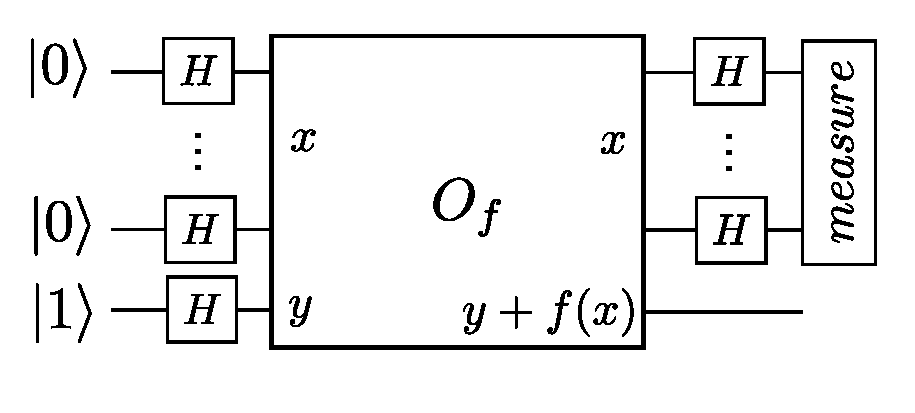
\includegraphics[width=.6\textwidth]{deutsch_josza.pdf}
\end{figure}
\end{center}

Let us walk through the steps of the algorithm for $n=1$.
In this case, either $f$ is constant and $f(0)=f(1)=b$, 
or $f$ is balanced and $f(0)=b$ while $f(1)=1-b$.
For all binary numbers we write $\overline{x}=1-x$

To start with, Hadamard gates are applied:

\begin{align*}
    |01\rangle &\xrightarrow{H\otimes H} \left(\frac{|0\rangle+|1\rangle}{\sqrt{2}}\right)\otimes \left(\frac{|0\rangle-|1\rangle}{\sqrt{2}}\right)\\
    &= \left(\frac{|00\rangle+|10\rangle-|01\rangle-|11\rangle}{2}\right)
\end{align*}
Then, the oracle, which yields:
\begin{align*}
\frac{|0f(0)\rangle+|1f(1)\rangle-|0\overline{f(0)}\rangle-|1\overline{f(1)}\rangle}{2}
\end{align*}
Now let us distinguish the two cases:
\begin{itemize}
    \item if $f$ is constant, the application of $H\otimes I$ will yield:
\begin{align*}
\frac{|0f(0)\rangle+|1f(1)\rangle-|0\overline{f(0)}\rangle-|1\overline{f(1)}\rangle}{2}
&=\frac{|0b\rangle+|1b\rangle-|0\overline{b}\rangle-|1\overline{b}\rangle}{2}\\
&=\left(\frac{|0\rangle+|1\rangle}{\sqrt{2}}\right)\otimes \left(\frac{|b\rangle-|\overline{b}\rangle}{\sqrt{2}}\right)\\
&\xrightarrow[H\otimes I]{} |0\rangle \otimes \left(\frac{|b\rangle-|\overline{b}\rangle}{\sqrt{2}}\right)
\end{align*}
and therefore $0$ is measured.
\item if $f$ is balanced, then $f(0)=b$ and $f(1)=\overline{b}$ and:
\begin{align*}
\frac{|0f(0)\rangle+|1f(1)\rangle-|0\overline{f(0)}\rangle-|1\overline{f(1)}\rangle}{2}
&=\frac{|0b\rangle+|1\bar{b}\rangle-|0\overline{b}\rangle-|1b\rangle}{2}\\
&\xrightarrow[H\otimes I]{}
    \frac{\cancel{|0b\rangle}+|1b\rangle+\cancel{|0\bar{b}\rangle}-|1\bar{b}\rangle-\cancel{|0\overline{b}\rangle}-|1\overline{b}\rangle-\cancel{|0b\rangle}+|1b\rangle}{\sqrt{8}}\\
&= |1\rangle\otimes\left(\frac{|b\rangle-|\overline{b}\rangle}{\sqrt{2}}\right)
\end{align*}
\end{itemize}
\subsection{Quantum Fourier Transform}

\subsection{Phase Estimation}

\subsection{Overview: other algorithms and their speedup}



\section{What you will do in the TP: QPE and VQE for quantum chemistry}

\end{document}
